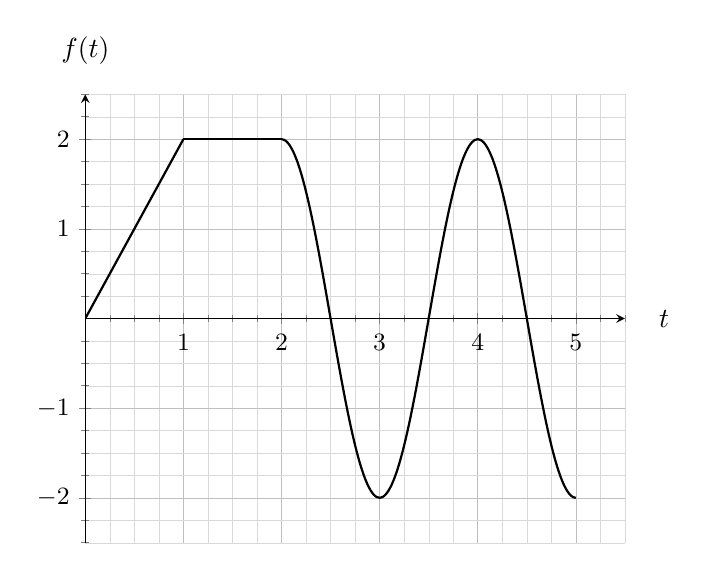
\begin{tikzpicture}
    \begin{axis}[
        grid=both,
        grid style={line width=.1pt, draw=gray!30},
        major grid style={line width=.2pt,draw=gray!50},
        every tick label/.append style={font=\small},
        axis x line = middle,
        axis y line = middle,
            every axis y label/.style={at={(ticklabel cs:1.15)}},
            %ytick = {-4, -2, -3, -1, 1, 2, 3, 4},
        y label style={at={(axis description cs:0,1.15)},anchor=north},
            ylabel = {$f(t)$},
            every axis x label/.style= {at ={(ticklabel cs:1)}},
            %xtick = {-4,-3,-2,-1,1,2,3,4},
            x label style={at={(axis description cs:1.1,.5)},anchor=east},
            xlabel = {$t$},
            xmax = 5.5, ymin = -2.5, ymax = 2.5,
            minor tick num = 3
    ]
    
        \addplot[thick,domain = 0:1] {2*x};
        \addplot[thick,domain = 1:2] {2};
        \addplot[thick,smooth,samples=100,domain = 2:5] {2*cos((180)*(x-2))};
    \end{axis}
\end{tikzpicture}